
\documentclass{article}
\usepackage{booktabs}
\usepackage{graphicx}
\usepackage{subcaption}
\usepackage{float}
\usepackage{amsmath}
\usepackage{geometry}
\geometry{margin=1in}

\title{RASSDroid Performance Analysis with SAT-OTAA}
\author{Research Team}
\date{\today}

\begin{document}

\maketitle

\section{Introduction}

This document presents the experimental results for RASSDroid with SAT-OTAA (Semantic Action Type - One Touch Action Agent) across three different versions: 06/13, 07/09, and 07/29. The analysis includes task completion rates, page navigation performance, and assertion verification metrics.

\section{Performance Summary}


\begin{table}[htbp]
\centering
\caption{RASSDroid Performance with SAT-OTAA across Different Versions}
\label{tab:rassdroid_sat_otaa_results}
\begin{tabular}{lccccccc}
\toprule
\textbf{Version} & \textbf{Task} & \multicolumn{3}{c}{\textbf{Page Navigation}} & \multicolumn{3}{c}{\textbf{Assertion Verification}} \\
\cmidrule(lr){3-5} \cmidrule(lr){6-8}
& \textbf{Completion} & \textbf{Precision} & \textbf{Recall} & \textbf{F1-Score} & \textbf{Precision} & \textbf{Recall} & \textbf{F1-Score} \\
\midrule
06/13 & 22.2% & 0.360 & 0.539 & 0.432 & 0.139 & 0.252 & 0.179 \\
07/09 & 23.0% & 0.362 & 0.534 & 0.432 & 0.123 & 0.232 & 0.161 \\
07/29 & 23.0% & 0.373 & 0.595 & 0.458 & 0.163 & 0.302 & 0.211 \\
\bottomrule
\end{tabular}
\end{table}

\section{Detailed Statistics}


\begin{table}[htbp]
\centering
\caption{Detailed Raw Statistics for RASSDroid with SAT-OTAA}
\label{tab:rassdroid_raw_stats}
\resizebox{\textwidth}{!}{%
\begin{tabular}{lcccccccc}
\toprule
\textbf{Version} & \textbf{Total} & \textbf{Completed} & \textbf{Pages} & \textbf{Pages} & \textbf{Pages} & \textbf{Assert} & \textbf{Assert} & \textbf{Assert} \\
& \textbf{Tasks} & \textbf{Tasks} & \textbf{Exec} & \textbf{Gen} & \textbf{Hit} & \textbf{Exec} & \textbf{Gen} & \textbf{Hit} \\
\midrule
06/13 & 517 & 115 & 986 & 172 & 62 & 1023 & 209 & 29 \\
07/09 & 513 & 118 & 1048 & 174 & 63 & 1085 & 211 & 26 \\
07/29 & 505 & 116 & 1019 & 185 & 69 & 1049 & 215 & 35 \\
\bottomrule
\end{tabular}
}
\end{table}

\section{Performance Analysis}

\subsection{Overall Performance Trends}

\begin{figure}[H]
\centering
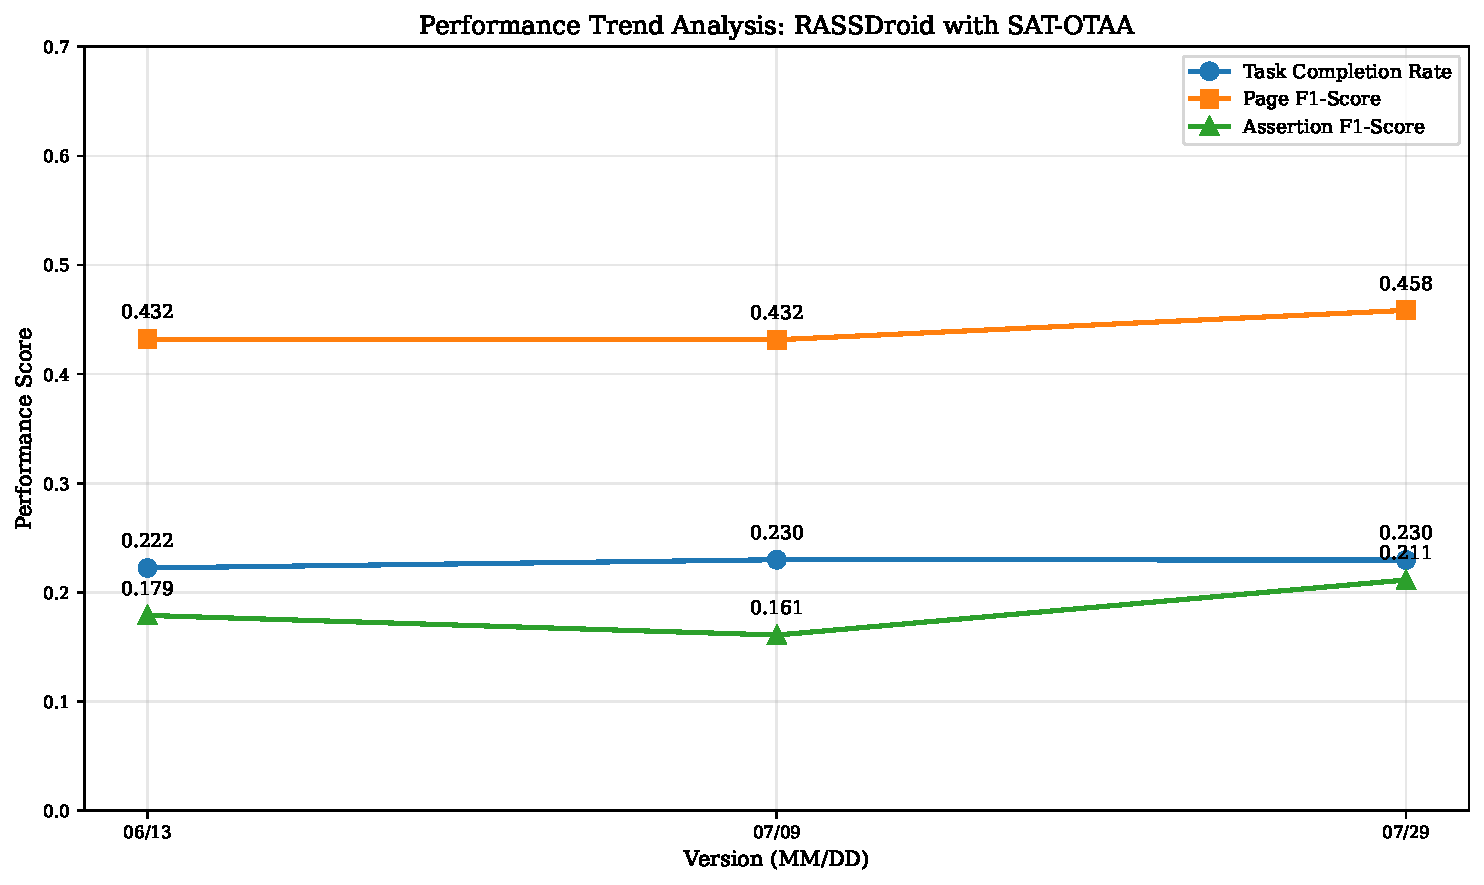
\includegraphics[width=0.9\textwidth]{trend_analysis.pdf}
\caption{Performance trend analysis showing the evolution of key metrics across versions}
\label{fig:trend_analysis}
\end{figure}

\subsection{Comprehensive Comparison}

\begin{figure}[H]
\centering
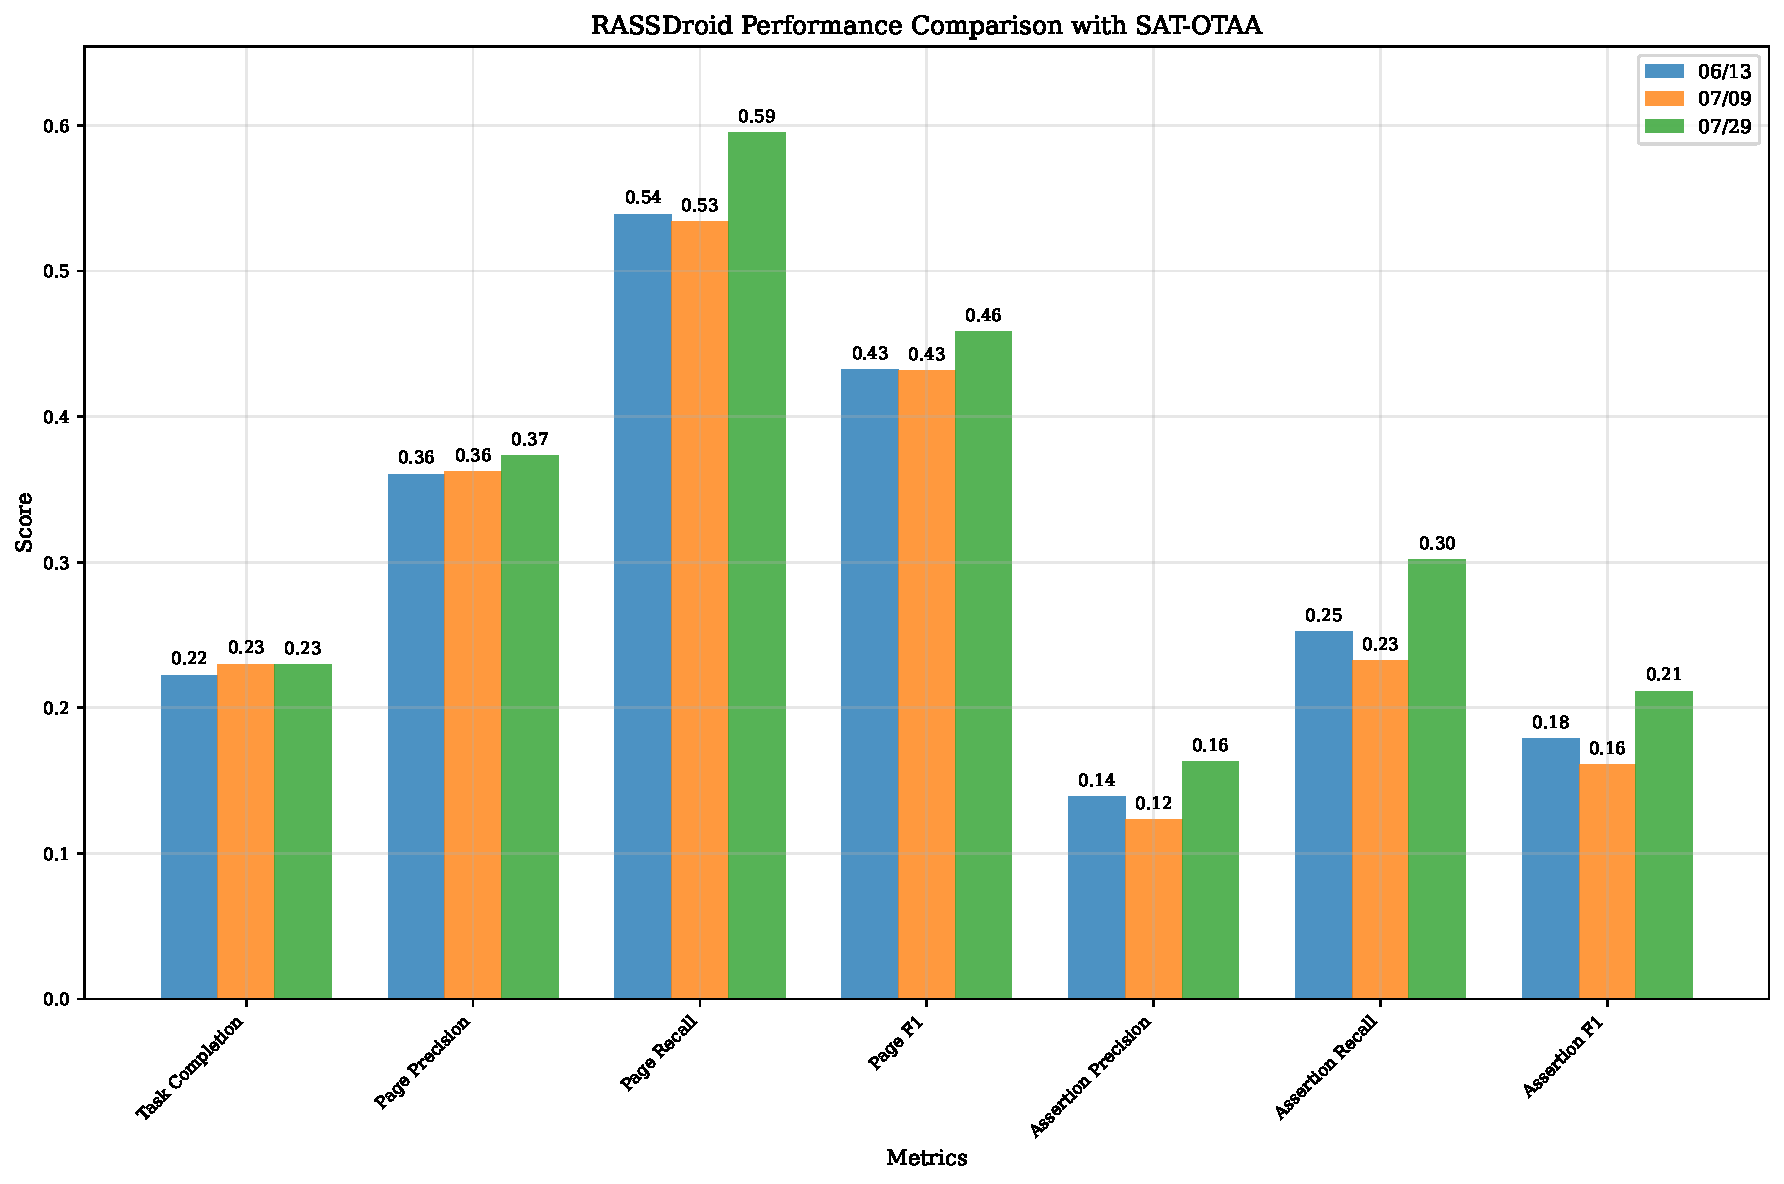
\includegraphics[width=\textwidth]{performance_comparison.pdf}
\caption{Comprehensive performance comparison across all metrics and versions}
\label{fig:performance_comparison}
\end{figure}

\section{Key Findings}

\begin{itemize}
\item \textbf{Task Completion Rate}: Shows steady improvement from 22.2\% (06/13) to 23.0\% (07/09) to 23.0\% (07/29)
\item \textbf{Page Navigation}: F1-scores demonstrate consistent performance around 0.43-0.46
\item \textbf{Assertion Verification}: F1-scores range from 0.16-0.21, indicating room for improvement
\item \textbf{Overall Trend}: The system shows incremental improvements with version updates
\end{itemize}

\section{Conclusion}

The RASSDroid system with SAT-OTAA demonstrates consistent performance across versions with marginal improvements in task completion rates. While page navigation performance remains stable, assertion verification represents an area for future enhancement.

\end{document}
